\documentclass{scsSimAUDPaperFormat}
% Beginning of preable.
% Ensure that the copyright notice matches the conference/symposium.
\copyrightnotice{
	SimAUD 2020 May 25-27 Vienna, Austria
	
	\copyright\,2020 Society for Modeling \& Simulation International (SCS)
}
% Load basic packages
\usepackage{balance}		% to better equalize the last page
\usepackage{graphics}		% for EPS, load graphicx instead
\usepackage{times}			% comment if you want LaTeX's default font
\usepackage{url}			% llt: nicely formatted URLs
\usepackage{dblfloatfix}	% allow placement of a page-width figure at top or bottom of page
% llt: Define a global style for URLs, rather that the default one

\makeatletter
\def\url@leostyle{%
  \@ifundefined{selectfont}{\def\UrlFont{\sf}}{\def\UrlFont{\small\bf\ttfamily}}}
\makeatother
\urlstyle{leo}

% To make various LaTeX processors do the right thing with page size.
\def\pprw{8.5in}
\def\pprh{11in}
\special{papersize=\pprw,\pprh}
\setlength{\paperwidth}{\pprw}
\setlength{\paperheight}{\pprh}
\setlength{\pdfpagewidth}{\pprw}
\setlength{\pdfpageheight}{\pprh}

% Make sure hyperref comes last of your loaded packages,
% to give it a fighting chance of not being over-written,
% since its job is to redefine many LaTeX commands.
\usepackage[pdftex]{hyperref}
\hypersetup{
pdftitle={SCS Conference Proceedings Format},
pdfauthor={LaTeX},
pdfkeywords={SCS, proceedings, archival format},
bookmarksnumbered,
pdfstartview={FitH},
colorlinks,
citecolor=black,
filecolor=black,
linkcolor=black,
urlcolor=black,
breaklinks=true,
}

% create a shortcut to typeset table headings
\newcommand\tabhead[1]{\small\textbf{#1}}

% create an affilitation superscript
\newcommand{\affiliation}[1]{\ensuremath{^{\textrm{#1}}}}

% End of preamble. Here comes the document.

\begin{document}
\title{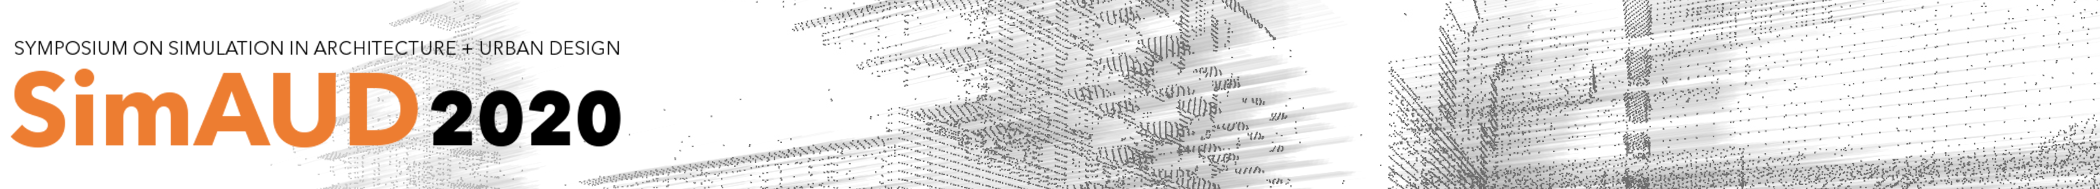
\includegraphics[width=1.0\textwidth]{SimAUDLogo.png}\\\quad\\SCS-SimAUD Conference Proceedings Format}

% Replace "UniversityA", "CompanyA", "UniversityB" with institution-specific abbreviations.
\def\UniversityA{\affiliation{1}} 
\def\CompanyA{\affiliation{2}}
\def\UniversityB{\affiliation{3}}

\author{
	First Author Name\UniversityA
	,
	Second Author Name\CompanyA
	,
	Third Author Name\UniversityB
	\,and
	Fourth Author Name\CompanyA
	\\
	\\
\affaddr{\UniversityA}{Affiliation, City, Country, e-mail address}\\
\affaddr{\CompanyA}{Affiliation, City, Country, e-mail address}\\
\affaddr{\UniversityB}{Affiliation, City, Country, e-mail address}	
}

\maketitle

\begin{abstract}
This sample paper describes the formatting requirements for Conference Proceedings, and this sample file offers recommendations on writing for the worldwide readership. Please review this document even if you have submitted to SCS conferences before because some format details have changed relative to previous years.
\end{abstract}

\keywords{
	Guides; instructions; author's kit; conference publications;
	keywords should be separated by a semi-colon.	
	\textcolor{red}{Optional section to be included in your final version, but strongly encouraged..}
}

% ACM Classification Keywords
\category{I.6.1}{SIMULATION AND MODELING (e.g. Model Development). }
See: \url{http://www.acm.org/about/class/1998/} for more information and the full list of ACM classifiers and descriptors.
\textcolor{red}{Optional section to be included in your final version, but strongly encouraged.}

\section{Introduction}

This format is to be used for submissions that are published in the conference proceedings. We wish to give this volume a consistent, high-quality appearance. We therefore ask that authors follow some simple guidelines. In essence, you should format your paper exactly like this document. The easiest way to do this is simply to download a template from the conference web site, and replace the content with your own material. To obtain WORD DOC and Latex templates, please refer to the Author’s Kit on the SCS website.

\section{Page Size and Columns}

On each page your material should fit within a rectangle of 18 x 23.5 cm (7 in. x 9.25 in.), centered on a US letter page (21.59 x 27.94 cm; 8.5x11 inches), beginning 1.9 cm (.75 in.) from the top of the page, with a .85 cm (.33 in.) space between two 8.4 cm (3.3 in.) columns. Right margins should be justified (i.e. fully-justified), not ragged (except for the references section). Beware, especially when using this template on a Macintosh, Word can change these dimensions in unexpected ways. Please be sure your pdf is US letter and not A4. If your pdf are formatted for A4, the submission will be returned to you to fix within 2 days.

\section{Typeset Text}

Prepare your submissions on a word processor or typesetter. Please
note that page layout may change slightly depending upon the printer
you have specified. \LaTeX\ sometimes will create overfull lines
that extend into columns. To attempt to combat this, the .cls
file has a command, {\textbackslash}sloppy, that essentially asks
\LaTeX\ to prefer underfull lines with extra whitespace. For more
details on this, and info on how to control it more finely, check out
{\url{http://www.economics.utoronto.ca/osborne/latex/PMAKEUP.HTM}}.

\subsection{Title and Authors}

Your paper’s title, authors and affiliations should run across the full width of the page in a single column 17.8 cm (7 in.) wide. The title should be in Ariel 18-point bold; use Helvetica if Ariel is not available. Authors’ names should be in Times New Roman 12-point bold, and affiliations in Times New Roman 12-point (not bold, nor italic). 

Please use full international addresses. Leave two 10-pt lines of white spaces below the last line of affiliations. 

For the anonymous review copy of the manuscript, omit the authors’ names and affiliations. In place of the names, insert the submission number assigned by the online submission system.

\subsection{Abstract and Keywords}

Every submission should begin with an abstract of about 150 words (max. 200), followed by a set of keywords. The abstract and keywords should be placed in the left column of the first page under the left half of the title. The abstract should be a concise statement of the problem, approach and conclusions of the work described. It should clearly state the paper's contribution to the field of M\&S.

The first set of keywords will be used to index the paper in the proceedings. The second set are used to catalogue the paper in the ACM Digital Library. The latter are entries from the ACM Classification System \cite{acm_categories}.

\subsection{Normal or Body Text}

Please use a 10-point Times New Roman font or, if this is unavailable, another proportional font with serifs, as close as possible in appearance to Times New Roman 10-point. The Press 10-point font available to users of Script is a good substitute for Times New Roman. On a Macintosh, use the font named Times not Times New Roman. Please use sans-serif or non-proportional fonts only for special purposes, such as headings or source code text.

\subsection{First Page Copyright Notice}

This template has the correct SCS copyright notice in place (see page 1, bottom of column 1). Copyright will be held by SCS. Accepted work-in-progress and papers will be distributed in the Conference Publications. They will also be placed in the ACM Digital Library, as well as other prominent digital libraries, where they will remain accessible to thousands of researchers and practitioners worldwide. Leave 3 cm (1.25 in.) of blank space for the copyright notice at the bottom of the left column of the first page. In this template a floating text box will automatically generate the required space.

\subsection{Subsequent Pages}

On pages beyond the first, start at the top of the page and continue in double-column format. The two columns on the last page should be as close as possible to equal length.

\begin{figure}[!h]
\centering
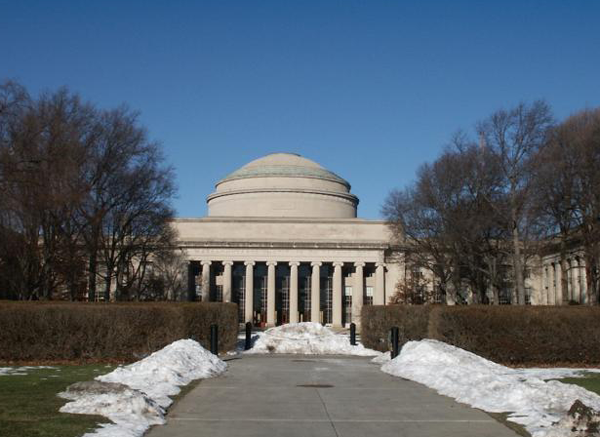
\includegraphics[width=0.9\columnwidth]{Figure1}
\caption{With caption below, be sure to have a good resolution image (see below for image preparation instructions).}
\label{fig:figure1}
\end{figure}

\subsection{References and Citations}

Use a numbered list of references at the end of the article, ordered alphabetically by first author, and referenced by numbers in brackets [2, 4, 5, 7]. Kindly make the text of this section left-justified/ragged-right (instead of fully-justified as in the rest of the document), so that the increasing number of references/citations with web addresses/URLs do not have large word and letter spacing. For papers from conference proceedings, include the title of the paper and an abbreviated name of the conference (e.g., for Interact 2003 proceedings, use \textit{Proc. Interact 2003}). Do not include the location of the conference or the exact date; do include the page numbers if available. See the examples of citations at the end of this document. Within this template file, use the \texttt{References} style
for the text of your citation.

Your references should be published materials accessible to the public. Internal technical reports may be cited only if they are easily accessible (i.e., you provide the address for obtaining the report within your citation) and may be obtained by any reader for a nominal fee. Proprietary information may not be cited. Private communications should be acknowledged in the main text, not referenced (e.g., “[Robertson, personal communication]”).

\begin{table}
  \centering
  \begin{tabular}{|c|c|c|}
    \hline
    \tabhead{Objects} &
    \multicolumn{1}{|p{0.3\columnwidth}|}{\centering\tabhead{Caption --- pre-2002}} &
    \multicolumn{1}{|p{0.4\columnwidth}|}{\centering\tabhead{Caption --- 2003 and afterwards}} \\
    \hline
    Tables & Above & Below \\
    \hline
    Figures & Below & Below \\
    \hline
  \end{tabular}
  \caption{Table captions should be placed below the table.}
  \label{tab:table1}
  \hfill \break
  \centering
  \begin{tabular}{|c|c|c|c|c|}
	\hline
	\tabhead{} &
	\multicolumn{1}{|p{0.15\columnwidth}|}{\centering\tabhead{Anyone}} &
	\multicolumn{1}{|p{0.15\columnwidth}|}{\centering\tabhead{SN}} &
	\multicolumn{1}{|p{0.15\columnwidth}|}{\centering\tabhead{Specific}} &
	\multicolumn{1}{|p{0.15\columnwidth}|}{\centering\tabhead{No one}} \\
	\hline
	\textbf{Flight} & 45\% & 34\% & 18\% & 3\% \\
	\hline
	\textbf{City} & 47\% & 35\% & 14\% & 3\% \\
	\hline
  \end{tabular}
  \caption{Sharing travel plans}
  \label{tab:table2}
\end{table}

\section{Sections}

Headings of subsections should be in Ariel 9-point bold, all in capitals. Sections should be numbered. 

\subsection{Subsections}

Headings of subsections should be in Ariel 9-point bold with
initial letters capitalized. Note: For sub-sections and sub-subsections, a word like \emph{the} or \emph{of} is not capitalized unless it is the first word of the heading.

\subsubsection{Sub-subsections}

Headings for sub-subsections should be in Ariel 9-point italic
with initial letters capitalized. Standard {\textbackslash}section,
{\textbackslash}subsection, and {\textbackslash}subsubsection commands
will work fine.

\begin{figure*}[ht!]
	\centering
	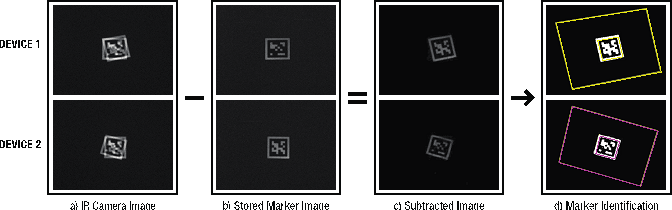
\includegraphics[width=1.0\textwidth]{Figure2}
	\centering
	\caption{Sample of a wide figure. Be sure to place at the top of the page or bottom of the page.}
	\centering
	\label{fig:figure2}
\end{figure*}

\section{Figures/Captions}

Place figures and tables at the top or bottom of the appropriate column or columns, on the same page as the relevant text (see Figure~\ref{fig:figure1}). 

A figure or table may extend across both columns to a maximum width of 17.78 cm (7 in.). Captions should be Times New Roman 9-point bold (Caption Style in this template file). They should be numbered (e.g., “Table 1” or “Figure 2”), centered and placed beneath the figure or table. Please note that the words “Figure” and “Table” should be spelled out (e.g. use “Figure” rather than “Fig.”) wherever they occur. 

Papers and notes may use color figures, which are included in the page limit; the figures must be readable when printed in black and white in the proceedings.

The paper may be accompanied by a short video figure up to five minutes in length. However, the paper should stand on its own without the video figure, as the video may not be available to everyone who reads the paper.


\subsection{Image Preparation}

Be sure your image has been resized to the appropriate printing resolution (usually 300 dpi).

\subsection{Table Style}
Tables should be prepared with consistent styling as specified with the cls file with captions marked clearly for interpretation. Long tables are recommended to be introduced by interrupting the multicolumn temporarily and/or as according to Figure ~\ref{fig:figure2}.
\section{Language, Style and Content}

The written and spoken language of SCS is English. Spelling and punctuation may use any dialect of English (e.g., British, Canadian, US, etc.) provided this is done consistently. Hyphenation is optional. To ensure suitability for an international audience, please pay attention to the following (note that while the items in this list are bulleted numbered lists are allowed):

\begin{itemize}
\item Write in a straightforward style.
\item Try to avoid long or complex sentence structures.
\item Briefly define or explain all technical terms that may be unfamiliar to readers.
\item Explain all acronyms the first time they are used in your text---e.g.,``Digital Signal Processing (DSP)''.
\item Explain local references (e.g., not everyone knows all city names in a particular country).
\end{itemize}



\begin{itemize}
\item Explain ``insider'' comments. Ensure that your whole audience understands any reference whose meaning you do not describe (e.g., do not assume that everyone has used a Macintosh or a particular application).
\item Explain colloquial language and puns. Understanding phrases like ``red herring'' may require a local knowledge of English. Humor and irony are difficult to translate.
\item Use unambiguous forms for culturally localized concepts, such as times, dates, currencies and numbers (e.g., ``1-5-97'' or ``5/1/97'' may mean 5 January or 1 May and ``12/10/11'' can be even more confusing, and ``seven o'clock'' may mean 7:00 am or 19:00). For currencies, indicate equivalences---e.g., ``Participants were paid 10,000 lire, or roughly \$5.''
\item Be careful with the use of gender-specific pronouns (he, she) and other gendered words (chairman, manpower, man-months). Use inclusive language that is gender-neutral (e.g., she or he, they, s/he, chair, staff, staff-hours, person-years). See~\cite{Schwartz:1995:GBF} for further advice and examples regarding gender and other personal attributes.
\item If possible, use the full (extended) alphabetic character set for names of persons, institutions, and places (e.g., Gr{\o}nb{\ae}k, Lafreni\'ere, S\'anchez, Universit{\"a}t, Wei{\ss}enbach, Z{\"u}llighoven, \r{A}rhus, etc.). These characters are already included in most versions of Times, Helvetica, and Arial fonts.
\end{itemize}

\section{Page Numbering, Headers and Footers}

Your final submission MUST NOT contain any footer or header information at the top or bottom of each page. The submissions will be paginated in a determined order by the chairs and page numbers added to the pdf during the compiling, indexing, and pagination processes. Comment out the {\textbackslash}pagenumbering command at the top of the document to remove page numbers.

\section{Producing and Testing PDF Files}

We recommend that you produce a PDF version of your submission well
before the final deadline. Test your PDF file by viewing or printing it with the same software we
will use when we receive it, Adobe Acrobat Reader Version 7. This is
widely available at no cost from~\cite{acrobat}. Note that most
reviewers will use a North American/European version of Acrobat
reader, which cannot handle documents containing non-North American or
non-European fonts (e.g. Asian fonts). Please therefore do not use
Asian fonts, and verify this by testing with a North American/European
Acrobat reader (obtainable as above). Something as minor as including
a space or punctuation character in a two-byte font can render a file
unreadable.

\section{Conclusion}

It is important that you write for the SCS audience. Please read previous years’ Proceedings to understand the writing style and conventions that successful authors have used. It is particularly important that you state clearly what you have done, not merely what you plan to do, and explain how your work is different from previously published work, (i.e. what is the unique contribution that your work makes to the field) ? Please consider what the reader will learn from your submission, and how they will find your work useful. If you write with these questions in mind, your work is more likely to be successful, both in being accepted into the Conference, and in influencing the work of our field.

\section*{ACKNOWLEDGMENTS}

Sample Text: We thank all volunteers, and all publications support and staff, who wrote and provided helpful comments on previous versions of this document. As well authors 1, 2, \& 3 gratefully acknowledge the grant from NSF (\# 1234 2012 ABC). This whole paragraph is just for example. Some of the references cited in this paper are included for illustrative purposes only.


\balance

% Balancing columns in a ref list is a bit of a pain because you
% either use a hack like flushend or balance, or manually insert
% a column break. http://www.tex.ac.uk/cgi-bin/texfaq2html?label=balance
% multicols doesn't work because we're already in two-column mode,
% and flushend isn't awesome, so we chose balance. See this
% for more info: http://cs.brown.edu/system/software/latex/doc/balance.pdf
%
% Note that in a perfect world balance wants to be in the first
% column of the last page.
%
% If balance doesn't work for you, you can remove that and
% hard-code a column break into the bbl file right before you
% submit:
%
% http://stackoverflow.com/questions/2149854/how-to-manually-equalize-columns-
% in-an-ieee-paper-if-using-bibtex
%

\bibliographystyle{scsBiblioStyle}
\bibliography{SampleReferences}

\centering
\large\bf The columns on the last page should be of approximately equal length.
\textcolor{red}{Remove these two lines from your final version.}


\end{document}
